%%%%%%%%%%%%%%%%%%%%%%%%%%%%%%%%%%%%%%%%%%%%%%%%%%%%%%%%
%%%%                                              %%%%%%
%%%%  Author: Peter Wilson                        %%%%%%
%%%%                                              %%%%%%
%%%%  Composite shells                        %%%%%%
%%%%                                              %%%%%%
%%%%%%%%%%%%%%%%%%%%%%%%%%%%%%%%%%%%%%%%%%%%%%%%%%%%%%%%


%fref generates automatically the respective abreviation/word in the text for the reference. You just have to define a label starting with the respective keyword.
%english: chap, sec, fig, eq, app
%deutsch: chap/kap, abs, abb, gl, anh
%see http://ctan.space-pro.be/tex-archive/macros/latex/contrib/fancyref/fancyref.pdf for more \section

%\onehalfspacing
%\setlength{\belowcaptionskip}{-17pt}

\chapter{Extension of shells to composite laminates}
\label{chap:chapter_composite_formulation_implementation}

\renewcommand{\Thema}{Extension of shells to composite laminates}

\lettrine[lines=2]{W}{ith} the ANDES-DKQ and DSG elements formulated and implemented for isotropic materials in the preceding chapters, extending them into composite laminate materials is now considered. The relevant theory is covered in chapter \ref{chap:chapter_2_1} which defines the scope of the formulation and implementation discussed here.

\section{Composite constitutive matrix formulation}
The formulation of orthotropic laminate composite is developed further by recalling the key results presented in chapter \ref{chap:chapter_2_1} and then transferring this into a form suitable for programming.

The general laminate shell stress resultants are related to the generalized mid-plane strains via the total combined constitutive matrix $\bar{\mathbf{C}}$ as follows:

\begin{equation} 
\bar{\mathbf{N}} = \bar{\mathbf{C}} \bar{\boldsymbol{\epsilon}} =
\begin{pmatrix}
N_{xx} \\
N_{yy} \\
N_{xy} \\
M_{xx} \\
M_{yy} \\
M_{xy} \\
Q_{x} \\
Q_{y} 
\end{pmatrix} 
=
\begin{pmatrix}
\mathbf{A} & \mathbf{B} & \mathbf{0} \\
\mathbf{B} & \mathbf{D} & \mathbf{0} \\
\mathbf{0}& \mathbf{0} & \alpha		\begin{pmatrix}
{A}_{44} & {A}_{45} \\
{A}_{45} & {A}_{55} 
\end{pmatrix} 
\end{pmatrix} 
\begin{pmatrix}
\epsilon_{xx} \\
\epsilon_{yy} \\
2\epsilon_{xy}\\
\kappa_{xx}\\
\kappa_{yy}\\
2\kappa_{xy} \\
2\epsilon_{yz} \\
2\epsilon_{xz}
\end{pmatrix}
\label{eqscomp_laminate_form1}
\end{equation}

The individual entries of the material sub matrices $\mathbf{A},\ \mathbf{B}$ and $\mathbf{C}$ are also recalled:

\begin{equation} 
A_{ij} = 
\int_{\frac{-h}{2}}^{\frac{h}{2}}
\bar{Q}_{ij}
\ dz\ ,
\hspace{5mm}
B_{ij} = 
\int_{\frac{-h}{2}}^{\frac{h}{2}}
\bar{Q}_{ij}\ z
\ dz\ ,
\hspace{5mm}
D_{ij} = 
\int_{\frac{-h}{2}}^{\frac{h}{2}}
\bar{Q}_{ij}\ z^2
\ dz
\label{eqscomp_laminate_form2}
\end{equation}

The entries $\bar{Q}_{ij}^{(k)}$ are rotated lamina stiffness's as per equation \ref{eqscomp_plane_stress_tensor_rotated}, related to the pure lamina-aligned stiffness's through the transformation matrix $\mathbf{T}$ of equation \ref{eqscomp11}.

By shifting perspective from abstract formulation to a more programmable approach, the total combined constitutive matrix $\bar{\mathbf{C}}$ of a laminate with $n$ laminae and total thickness $h$ can be decomposed into lamina contributions. Furthermore, the rotation of the lamina stiffness's can be postponed until each lamina constitutive matrix is assembled:

\begin{equation} 
 \bar{\mathbf{C}} = \sum_{k=1}^{n}  \mathbf{T}^{T(k)} {\mathbf{C}}^{(k)}  \mathbf{T}^{(k)}
\label{eqscomp_laminate_form3}
\end{equation}

The integral limits of the material sub matrices, which must only span the thickness of each lamina $k$, are updated accordingly:

\begin{equation} 
A_{ij}^{(k)} = 
\int_{z_k}^{z_{k+1}}
{Q}_{ij}^{(k)}
\ dz\ ,
\hspace{5mm}
B_{ij}^{(k)} = 
\int_{z_k}^{z_{k+1}}
{Q}_{ij}^{(k)}\ z
\ dz\ ,
\hspace{5mm}
D_{ij}^{(k)} = 
\int_{z_k}^{z_{k+1}}
{Q}_{ij}^{(k)}\ z^2
\ dz
\label{eqscomp_laminate_form4}
\end{equation} 

The above formulation details concern themselves with determining the stiffness matrix of a composite laminate shell. Recovery of lamina stresses also departs from the isotropic formulation, however, the details presented in \ref{Laminate strain and stress recovery} need little further development to be programmable, so they are not reproduced here.

\section{Implementation of composite constitutive matrix}
The general approach of extending both shell elements to composite laminate materials in a sensible and efficient manner was to abstract the composite specifics from the individual element formulation level as much as possible. This approach reduces duplicate coding and provides a centralized platform to develop and modify the composite capabilities of the elements in the future. Almost all of the composite laminate implementation was achieved by modifying the existing \texttt{ShellCrossSection} class and adding a new constitutive law class \texttt{LinearElasticOrthotropic2DLaw}. Naturally, access to the new functionality required minor modifications to the code of each shell element. With a view to illustrate the relationship between the individual elements and the \texttt{ShellCrossSection} and \texttt{LinearElasticOrthotropic2DLaw} classes, a generalized workflow of both elements is outlined in the following flowchart, highlighting only methods relevant to composites:

\begin{figure}[H]
	% Define block styles
	\tikzstyle{virtual} = [rectangle, minimum width=3cm, minimum height=1cm, text centered, draw=black, fill=orange!30]
	\tikzstyle{process} = [rectangle, minimum width=3cm, minimum height=1cm, text centered, draw=black, fill=white!30]
	\tikzstyle{arrow} = [thick,->,>=stealth]
	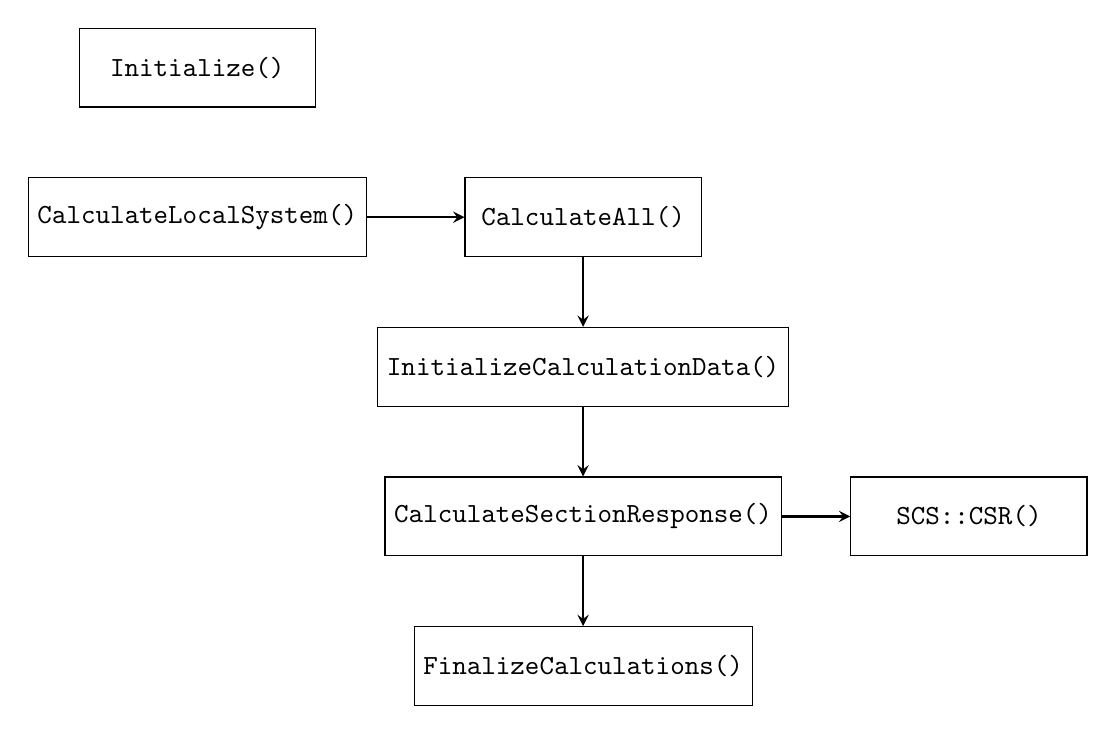
\begin{tikzpicture}[node distance = 1.9cm, auto]
	% Place nodes
	\node [process] (Initialize) {$\texttt{Initialize()}$};
	\node [process, below of=Initialize] (CalculateLocalSystem) {$\texttt{CalculateLocalSystem()}$};
	\node [process, right of=CalculateLocalSystem, xshift = 3cm] (CalculateAll) {$\texttt{CalculateAll()}$};
	\node [process, below of=CalculateAll, xshift = -0cm] (InitializeCalculationData) {$\texttt{InitializeCalculationData()}$};
	\node [process, below of=InitializeCalculationData, yshift = -0cm] (CalculateSectionResponse) {$\texttt{CalculateSectionResponse()}$};
	\node [process, below of=CalculateSectionResponse, yshift = -0cm] (FinalizeCalculations) {$\texttt{FinalizeCalculations()}$};
	\node [process, right of=CalculateSectionResponse, xshift = 3cm] (SCS) {$\texttt{SCS::CSR()}$};
	% Draw edges
	%\draw [arrow] (Initialize) -- (CalculateLocalSystem);
	\draw [arrow] (CalculateLocalSystem) -- (CalculateAll);
	\draw [arrow] (CalculateAll) -- (InitializeCalculationData);
	\draw [arrow] (InitializeCalculationData) -- (CalculateSectionResponse);
	\draw [arrow] (CalculateSectionResponse) -- (FinalizeCalculations);
	\draw [arrow] (CalculateSectionResponse) -- (SCS);
	\end{tikzpicture}
	\caption{High level overview of composite element workflow}
	\label{compositeworkflow}
\end{figure}

The key differences in the workflow presented above, compared to those previously illustrated, is the explicit inclusion of $\texttt{Initialize()}$ and $\texttt{ShellCrossSection::CalculateSectionResponse()}$, noted as $\texttt{SCS::CSR()}$, methods, which implement composite functionality. 

$\texttt{Initialize()}$ is called upon element creation, completely separate from $\texttt{CalculateLocalSystem()}$, and is responsible for reading in element material properties. Upon reading material data specified with the Kratos variable $\texttt{SHELL\_ORTHOTROPIC\_LAYERS}$, an instance of $\texttt{LinearElasticOrthotropic2DLaw}$ is created and assigned to the $\texttt{ShellCrossSection}$, followed by a call to the $\texttt{ShellCrossSection}$ method $\texttt{ShellCrossSection::ParseOrthotropicPropertyMatrix()}$ is called which parses and stores the orthotropic material data for all laminae. The checking of $\texttt{SHELL\_ORTHOTROPIC\_LAYERS}$ and parsing of orthotropic material data is performed entirely within the $\texttt{ShellCrossSection}$ class, which facilitates un-invasive integration into shell elements and also provides centralization for further composite development should the need arise.

Following the call of $\texttt{Initialize()}$, $\texttt{CalculateLocalSystem()}$ is called to compute the element-specific stiffness matrix. The ANDES-DKQ and DSG specifics of $\texttt{CalculateLocalSystem()}$ and it's subsequent calls are detailed in their respective chapters, the focus here are specifics relating to composite laminates. Logically, the call of $\texttt{CalculateSectionResponse()}$ is relevant, itself calling the $\texttt{ShellCrossSection}$ function $\texttt{ShellCrossSection::CalculateSectionResponse()}$.

The $\texttt{ShellCrossSection}$ method $\texttt{ShellCrossSection::CalculateSectionResponse()}$ serves to calculate the total laminate constitutive matrix $\bar{mathbf{C}}$ by 'stacking' the results of each lamina together. A loop is established over all laminae $k$, with each iteration retrieving the raw laminae stiffnesses $\mathbf{Q}^{(k)}$, integrating and assembling them into a lamina constitutive matrix $\mathbf{C}^{(k)}$ and then transforming them according to the stacking sequence of the lamina in the laminate. At the end of this method, the total laminate constitutive matrix $\bar{mathbf{C}}$ is assembled and suitable for use in element-specific methods to determine the stiffness matrix. 

A summary of the above flowchart and commentary is presented in the generalized composite shell element stiffness matrix pseudocode below:

\begin{algorithm}
	\onehalfspacing
	\caption{Generalized composite shell element stiffness matrix pseudocode}\label{general composite shell pseudocode}
	\begin{algorithmic}[1]
		\Require Orthotropic laminate material data specified
		\State \textbf{call} $\texttt{Initialize()}$
		\State \hspace{\algorithmicindent}\textbf{if} $materialProperties$ has orthotropic laminate data \textbf{then}
		\State \hspace{\algorithmicindent} \hspace{\algorithmicindent} Create and assign $\texttt{LinearElasticOrthotropic2DLaw}$
		\State \hspace{\algorithmicindent} \hspace{\algorithmicindent} Parse composite material data in $\texttt{ShellCrossSection}$
		\State \hspace{\algorithmicindent}\textbf{end if}
		\State \textbf{call} $\texttt{CalculateLocalSystem()}$
		\State \hspace{\algorithmicindent}Perform element-specific calculations (may enter Gauss loop)
		\State \hspace{\algorithmicindent}\textbf{call} $\texttt{CalculateSectionResponse}()$
		\State \hspace{\algorithmicindent}\hspace{\algorithmicindent} \textbf{call} $\texttt{ShellCrossSection::CalculateSectionResponse}()$
		\State \hspace{\algorithmicindent} \hspace{\algorithmicindent} \hspace{\algorithmicindent} \textbf{while} ($k$ < number of laminae) \textbf{do}
		\State \hspace{\algorithmicindent} \hspace{\algorithmicindent} \hspace{\algorithmicindent} \hspace{\algorithmicindent}Retrieve stiffnesses of $k^{th}$ lamina $\mathbf{Q}^{(k)}$ from material law
		\State \hspace{\algorithmicindent} \hspace{\algorithmicindent} \hspace{\algorithmicindent} \hspace{\algorithmicindent}Assemble and integrate unrotated lamina constitutive matrix $\mathbf{C}^{(k)}$
		\State \hspace{\algorithmicindent} \hspace{\algorithmicindent} \hspace{\algorithmicindent} \hspace{\algorithmicindent}\textbf{if} $laminaOrientationAngle \neq 0$ \textbf{then}
		\State \hspace{\algorithmicindent} \hspace{\algorithmicindent} \hspace{\algorithmicindent} \hspace{\algorithmicindent} \hspace{\algorithmicindent} Transform $\mathbf{C}^{(k)}$ into $\bar{\mathbf{C}}^{(k)}$
		\State \hspace{\algorithmicindent} \hspace{\algorithmicindent} \hspace{\algorithmicindent} \hspace{\algorithmicindent}\textbf{end if}
		\State \hspace{\algorithmicindent} \hspace{\algorithmicindent} \hspace{\algorithmicindent} \hspace{\algorithmicindent}Add lamina $\bar{\mathbf{C}}^{(k)}$ to laminate $\bar{\mathbf{C}}$
		\State \hspace{\algorithmicindent} \hspace{\algorithmicindent} \hspace{\algorithmicindent} \textbf{end while}
		\State \hspace{\algorithmicindent}Assemble element-specific stiffness matrix and finalize calculations
	\end{algorithmic}
\end{algorithm}

\section{Implementation of composite stress recovery}
The extension of both shell elements to handle composites also requires additional functionality to calculate composite stresses. As described in section \ref{Laminate strain and stress recovery}, the laminate stresses and strains require the generalized shell mid-plane strains be determined (refer to the stress and strain recovery sections of each element for details). With the mid-surface strains available, the new method $\texttt{CalculateLaminaStrains()}$, implemented in both elements, calculates and assembles the in-plane strains (as per equation \ref{eqscomp_strain_recovery2}) for the top and bottom surface of each lamina into a vector of vectors. It should be noted that a constant transverse shear strain is assumed across the laminate thickness, as per equation \ref{eqscomp_strain_recovery3}. Stresses of the top and bottom surfaces of each lamina are determined in the new method $\texttt{CalculateLaminaStresses()}$ from the rotated raw lamina stiffnesses and the lamina strains according to equation \ref{eqscomp_stress_recovery1}. Similar to the isotropic stress recovery already implemented, the lamina stresses can be output locally or globally oriented.

The follow pseudocode provides an overview of recovering stresses from the shell elements.

\begin{algorithm}
	\onehalfspacing
	\caption{Generalized composite shell element stress and strain recovery}
	\label{general composite shell stress pseudocode}
	\begin{algorithmic}[1]
		\Require $requestedQuantity = laminateStresses$, calculation of nodal displacements
		\State Perform all preliminary operations necessary to determine mid-plane $generalizedStrains$
		\While{Gauss loop}
		\State \hspace{\algorithmicindent}Calculate $B$ matrix at current $gaussPoint$
		\State $generalizedStrains$ = product$(B,\ localDisplacements)$
		\State \textbf{call} $\texttt{CalculateLaminaStrains}(data)$
		\State \hspace{\algorithmicindent}Determine $laminateStrains$ at top and bottom surface of each lamina 
		\State \textbf{call} $\texttt{CalculateLaminaStresses}(data)$
		\State \hspace{\algorithmicindent}Retrieve raw laminae stiffnesses
		\State \hspace{\algorithmicindent}\textbf{while} ($k$ < number of laminae) \textbf{do}
		\State \hspace{\algorithmicindent} \hspace{\algorithmicindent}$laminateStresses^{(2k)}$ = product$(\mathbf{C}^{(k)},\ laminateStrains^{(2k)})$
		\State \hspace{\algorithmicindent} \hspace{\algorithmicindent}$laminateStresses^{(2k+1)}$ = product$(\mathbf{C}^{(k},\ laminateStrains^{(2k+1)})$
		\State \hspace{\algorithmicindent}\textbf{while end}
		\If{$laminateStresses$ requires local orientation} 
		\State Rotate $laminateStresses$ to local orientation
		\EndIf
		\State Assemble $laminateStresses$ into $outputMatrix$
		\If{$laminateStresses$ requires global orientation} 
		\State Rotate $outputMatrix$ to global orientation
		\EndIf
		\State Interpolate $outputMatrix$ to standard Gauss points for visualisation
		\EndWhile
	\end{algorithmic}
\end{algorithm}

\section{Implementation of Tsai-Wu failure criterion}
The Tsai-Wu failure criterion described in section \ref{tsai wu background} is also implemented for both shell elements.